\documentclass[12pt,a4paper]{article}

% Packages
\usepackage[utf8]{inputenc}
\usepackage[T1]{fontenc}
\usepackage{graphicx}
\usepackage{hyperref}
\usepackage{amsmath}
\usepackage{booktabs}
\usepackage{xcolor}
\usepackage{listings}
\usepackage{float}
\usepackage{geometry}
\usepackage{titlesec}
\usepackage{fancyhdr}
\usepackage{natbib}
\usepackage{url}
\usepackage{enumitem}
\usepackage{tikz}
\usepackage{algorithm}
\usepackage{algpseudocode}
\usepackage{tcolorbox}
\usepackage{lipsum}
\usepackage{mdframed}
\usepackage{pifont}
\usepackage{wallpaper}

% Define colors
\definecolor{titlecolor}{RGB}{180,0,0}
\definecolor{framecolor}{RGB}{0,60,120}

% Page setup
\geometry{margin=1in}
\setlength{\parindent}{0pt}
\setlength{\parskip}{6pt}
\setlength{\headheight}{14.5pt}

% Header and footer
\pagestyle{fancy}
\fancyhf{}
\fancyhead[L]{Movie Recommendation System}
\fancyhead[R]{\thepage}
\renewcommand{\headrulewidth}{0.4pt}

% Title formatting
\titleformat{\section}{\normalfont\Large\bfseries}{\thesection}{1em}{}
\titleformat{\subsection}{\normalfont\large\bfseries}{\thesubsection}{1em}{}

% Code listing style


% Document info
\title{\LARGE \textbf{Movie Recommendation System}\\\large A Content-Based Approach Using TF-IDF and Cosine Similarity}
\author{Project Report}
\date{\today}

\begin{document}

% Title page
\begin{titlepage}
    % Create a decorative border using TikZ
    \begin{tikzpicture}[remember picture, overlay]
        % Outer frame
        \draw[line width=2pt, color=framecolor] 
            ([shift={(.5cm,.5cm)}]current page.south west) rectangle 
            ([shift={(-.5cm,-.5cm)}]current page.north east);
        
        % Inner frame
        \draw[line width=1pt, color=framecolor] 
            ([shift={(1cm,1cm)}]current page.south west) rectangle 
            ([shift={(-1cm,-1cm)}]current page.north east);
        
        % Corner decorations
        \foreach \corner in {north east, north west, south east, south west} {
            \draw[line width=1.5pt, color=titlecolor] 
                ([shift={(0.75cm,0.75cm)}]current page.\corner) -- 
                ([shift={(1.5cm,1.5cm)}]current page.\corner);
        }
   
        
    \end{tikzpicture}

    \centering
    \vspace*{2cm}
    {\LARGE \textbf{\textcolor{titlecolor}{Movie Recommendation System}}\par}
    \vspace{0.8cm}
    {\large A Content-Based Approach Using TF-IDF and Cosine Similarity\par}
    \vspace{4.5cm}
    
    \begin{tcolorbox}[width=0.9\textwidth, colback=white, colframe=framecolor, arc=5mm, boxrule=1pt]
        \centering
        
    \end{tcolorbox}
    
    \vfill
    \begin{tikzpicture}[remember picture, overlay]
        \node[anchor=south, yshift=2cm] at (current page.south) {
        };
    \end{tikzpicture}
\end{titlepage}
\thispagestyle{empty}

% Abstract
\clearpage
\thispagestyle{empty}

\begin{tikzpicture}[remember picture, overlay]
    % Add decorative elements to the abstract page
    \draw[line width=1pt, color=framecolor] 
        ([shift={(1cm,1cm)}]current page.south west) rectangle 
        ([shift={(-1cm,-1cm)}]current page.north east);
    
    % Add corner decorations
    \foreach \corner in {north east, north west, south east, south west} {
        \fill[color=titlecolor] ([shift={(0.8cm,0.8cm)}]current page.\corner) circle (0.15cm);
    }
    
    % Add a title for the abstract section
    \node[anchor=north, font=\Large\bfseries, text=framecolor] at ([yshift=-2cm]current page.north) {ABSTRACT};
    
   
   
\end{tikzpicture}

\vspace*{3cm}
\begin{mdframed}[linewidth=1pt, linecolor=framecolor, backgroundcolor=white, roundcorner=10pt, innerleftmargin=15pt, innerrightmargin=15pt, innertopmargin=15pt, innerbottommargin=15pt]
    \begin{abstract}
        \setlength{\parindent}{1em}
        \setlength{\parskip}{0.5em}
        \noindent{\large\textbf{\textcolor{titlecolor}{\ding{43}}}} This report presents a comprehensive analysis of a movie recommendation system built using content-based filtering techniques. The system leverages TF-IDF (Term Frequency-Inverse Document Frequency) vectorization and cosine similarity to provide personalized movie recommendations based on content features such as genres, keywords, cast, and plot descriptions.
        
        \noindent{\large\textbf{\textcolor{titlecolor}{\ding{43}}}} The report details the system architecture, implementation methodology, data processing techniques, and evaluation results. Visualizations are included to demonstrate the distribution of movie genres, similarity patterns between movies, and recommendation examples.
        
        \noindent{\large\textbf{\textcolor{titlecolor}{\ding{43}}}} The system is implemented as a web application with a Flask backend and responsive frontend, offering both API endpoints and a user-friendly interface for discovering movies.
    \end{abstract}
\end{mdframed}

\vspace{1cm}


\newpage
\tableofcontents
\newpage

% Introduction
\section{Introduction}

Recommendation systems have become an integral part of modern digital platforms, helping users discover content relevant to their interests from vast catalogs of options. In the context of movies, recommendation systems assist viewers in finding films they might enjoy based on various factors such as viewing history, preferences, and content characteristics.

This report details the development and implementation of a content-based movie recommendation system that analyzes movie attributes such as genres, keywords, cast, crew, and plot descriptions to identify similarities between films. By leveraging natural language processing techniques, specifically TF-IDF vectorization and cosine similarity, the system can suggest movies with content features similar to those a user has previously enjoyed.

\subsection{Project Objectives}

The primary objectives of this movie recommendation system project are:

\begin{itemize}
    \item To develop a content-based recommendation algorithm using TF-IDF and cosine similarity
    \item To implement RESTful API endpoints for accessing movie data and recommendations
    \item To analyze and visualize patterns in movie data and recommendation results
    \item To provide a seamless user experience across different devices
\end{itemize}

\subsection{Dataset}

The system utilizes the TMDB 5000 Movie Dataset, which contains comprehensive information about movies including titles, genres, keywords, cast, crew, and plot overviews. This dataset consists of approximately 5,000 movies from The Movie Database (TMDB) and provides rich textual content that can be processed and analyzed to identify similarities between movies based on their content features. The implementation also includes a fallback mechanism to create sample data when the TMDB dataset files are not available.

% Methodology
\section{Methodology}

The movie recommendation system employs a content-based filtering approach, which recommends items based on their features and attributes rather than user behavior or preferences. This section outlines the key methodological components of the system.

\subsection{Content-Based Filtering}

Content-based filtering recommends items by comparing the content of items rather than relying on user interactions. In this system, movies are represented as vectors in a high-dimensional space where each dimension corresponds to a term or feature extracted from the movie's attributes. The similarity between movies is then calculated based on the proximity of these vectors.

The advantages of content-based filtering include:

\begin{itemize}
    \item No cold-start problem for new items (movies can be recommended as soon as their features are available)
    \item Transparency in recommendations (the system can explain why a particular movie was recommended)
    \item Independence from user data (no need for user ratings or viewing history)
\end{itemize}

\subsection{TF-IDF Vectorization}

Term Frequency-Inverse Document Frequency (TF-IDF) is a numerical statistic that reflects the importance of a word in a document relative to a collection of documents. In the context of this system, each movie is treated as a document, and its attributes (genres, keywords, cast, crew, overview) are processed to extract terms.

The TF-IDF value increases proportionally to the number of times a word appears in the document but is offset by the frequency of the word in the corpus, which helps to adjust for the fact that some words appear more frequently in general.

Mathematically, TF-IDF is calculated as:

\begin{equation}
    \text{TF-IDF}(t, d, D) = \text{TF}(t, d) \times \text{IDF}(t, D)
\end{equation}

Where:
\begin{itemize}
    \item $t$ is the term
    \item $d$ is the document (movie)
    \item $D$ is the document collection (all movies)
    \item $\text{TF}(t, d)$ is the term frequency of $t$ in $d$
    \item $\text{IDF}(t, D)$ is the inverse document frequency of $t$ in $D$
\end{itemize}

\subsection{Cosine Similarity}

After representing movies as TF-IDF vectors, the system calculates the similarity between these vectors using cosine similarity. Cosine similarity measures the cosine of the angle between two vectors, providing a value between -1 and 1, where 1 represents identical vectors and -1 represents completely opposite vectors.

For two movies represented by vectors $A$ and $B$, the cosine similarity is calculated as:

\begin{equation}
    \text{similarity}(A, B) = \frac{A \cdot B}{||A|| \times ||B||}
\end{equation}

Where $A \cdot B$ is the dot product of vectors $A$ and $B$, and $||A||$ and $||B||$ are their Euclidean norms.

% Implementation
\section{Implementation}

This section details the technical implementation of the movie recommendation system, including the backend architecture, data processing pipeline, and frontend development.

\subsection{Technology Stack}

The system is built using the following technologies:

\begin{itemize}
    \item \textbf{Backend:} Python, Flask, NumPy, Pandas, scikit-learn
    \item \textbf{Data Processing:} TF-IDF Vectorization, Cosine Similarity
    \item \textbf{Frontend:} HTML, CSS, JavaScript
    \item \textbf{Visualization:} Matplotlib, Seaborn
    \item \textbf{Data Storage:} Pickle (for model serialization)
\end{itemize}

\subsection{Data Processing Pipeline}

The data processing pipeline consists of the following steps:

\begin{enumerate}
    \item \textbf{Data Loading:} The system first checks if the TMDB 5000 Movie Dataset files exist locally. If not found, it provides instructions to download them from Kaggle. The implementation also includes a fallback mechanism to create sample data when the dataset files are not available.
    \item \textbf{Data Cleaning:} Missing values are removed, and text fields are processed to extract relevant information.
    \item \textbf{Feature Extraction:} The system extracts and processes features from various movie attributes:
    \begin{itemize}
        \item Genres are extracted from the genres field
        \item Keywords are extracted from the keywords field
        \item Cast members (top 3) are extracted from the cast field
        \item Director is extracted from the crew field
        \item Overview text is processed to extract meaningful terms
    \end{itemize}
    \item \textbf{Tag Creation:} All extracted features are combined into a single "tags" field for each movie, with spaces removed and text converted to lowercase for better processing.
    \item \textbf{TF-IDF Vectorization:} The tags are converted into TF-IDF vectors using scikit-learn's TfidfVectorizer with a maximum of 5000 features and English stop words removed.
    \item \textbf{Similarity Calculation:} Cosine similarity is calculated between all movie vectors to create a similarity matrix.
    \item \textbf{Model Serialization:} The processed movie data and similarity matrix are serialized using pickle for efficient loading during runtime.
\end{enumerate}

\subsection{Backend Architecture}

The backend is implemented using Flask, a lightweight Python web framework. It provides the following API endpoints:

\begin{itemize}
    \item \textbf{GET /}: Serves the main page of the application
    \item \textbf{GET /search}: Serves the search page
    \item \textbf{GET /api/search}: Searches for movies based on a query string
    \item \textbf{GET /api/movies}: Returns a list of all movies in the dataset
    \item \textbf{GET /api/recommend}: Returns movie recommendations based on a given movie name
\end{itemize}

The backend includes robust error handling for loading the preprocessed movie data and similarity matrix from pickle files at startup. If the model files don't exist, the system automatically creates sample data using the sample\_data.py module. This ensures the application can run even without the full TMDB dataset, which is particularly useful for testing and demonstration purposes.

The search functionality includes both exact and flexible matching to improve user experience. When a recommendation request is received, the system finds the index of the specified movie in the dataset, retrieves the corresponding row from the similarity matrix, sorts the similarity scores, and returns the top N most similar movies.

\subsection{Frontend Implementation}

The frontend is implemented using HTML, CSS, and JavaScript. It provides a responsive user interface with the following features:

\begin{itemize}
    \item Search functionality to find movies
    \item Display of movie recommendations with posters and titles
\end{itemize}

The frontend communicates with the backend API to retrieve movie data and recommendations, which are then displayed to the user in an intuitive and visually appealing manner.

% Data Analysis and Visualization
\section{Data Analysis and Visualization}

This section presents various analyses and visualizations of the movie dataset and recommendation system results. The visualizations are generated using Matplotlib and Seaborn libraries and are saved in the static/visualizations directory for display in the report and web interface.

\subsection{Genre Distribution}

The distribution of movie genres in the dataset provides insights into the content diversity and potential recommendation patterns. Figure \ref{fig:genre_distribution} shows the frequency of different genres in the dataset. The genres are extracted from the tags field using regular expression pattern matching to identify common genre terms.

\begin{figure}[H]
    \centering
    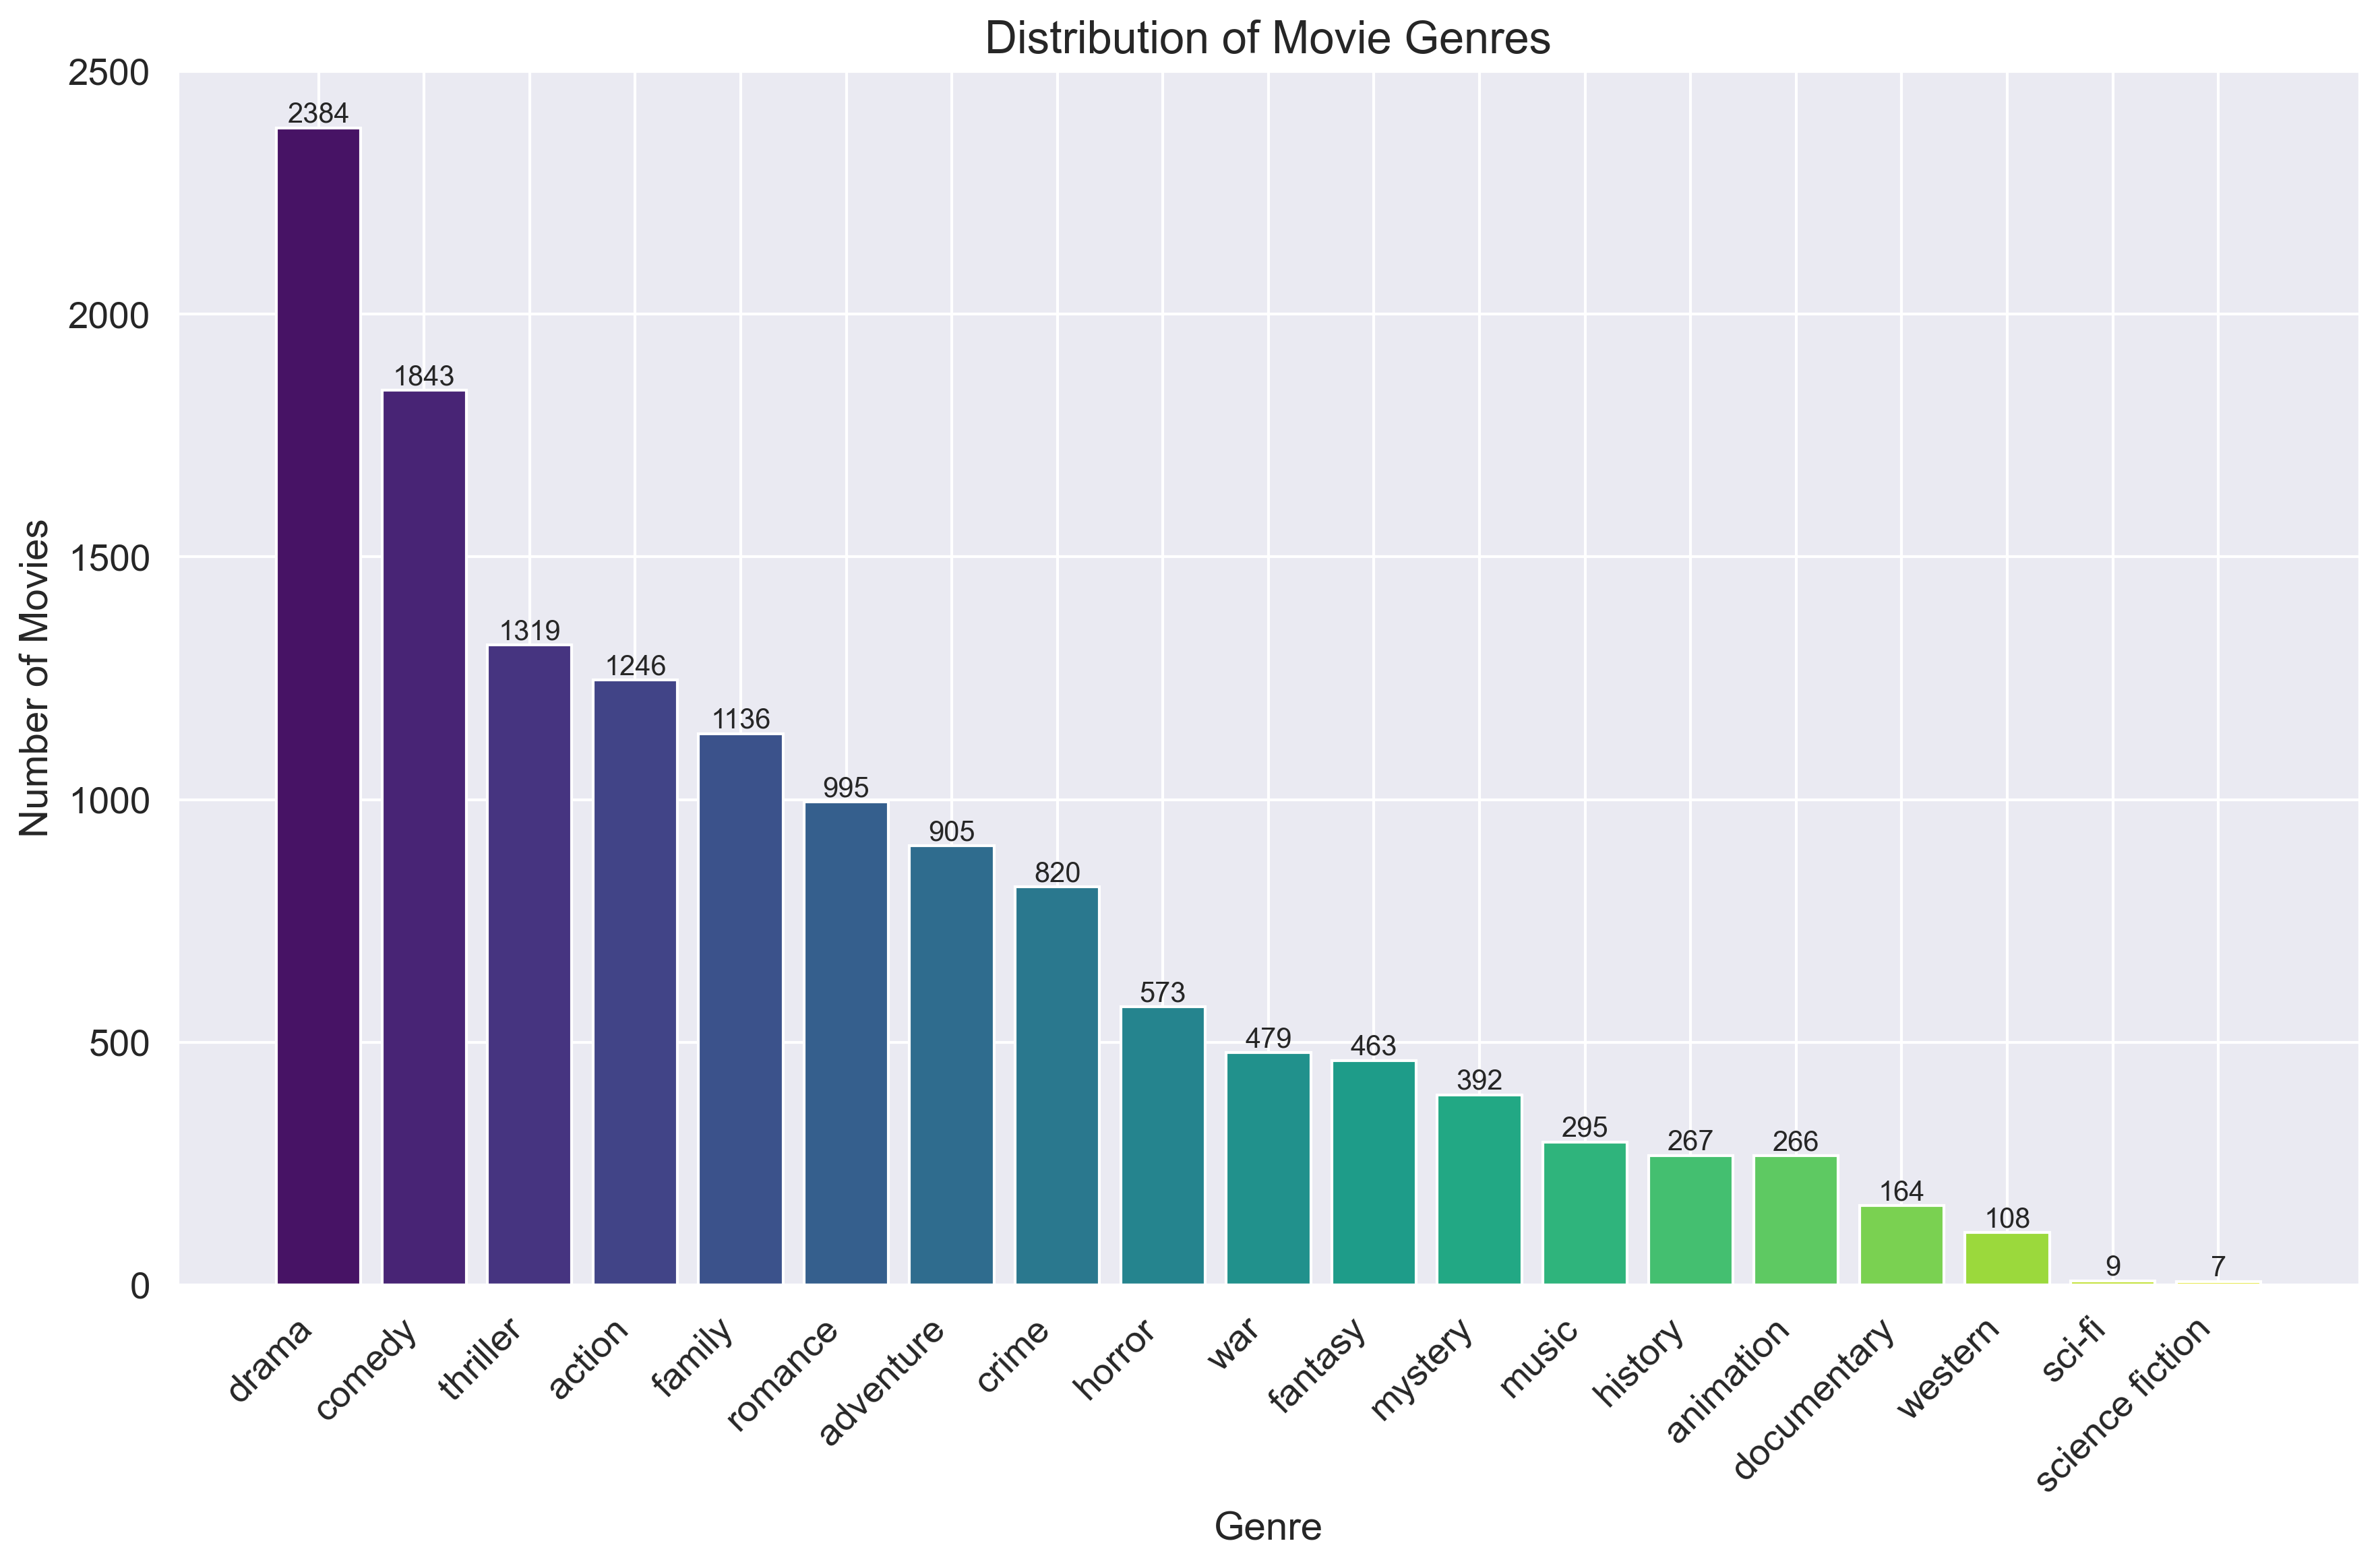
\includegraphics[width=0.9\textwidth]{static/visualizations/genre_distribution.png}
    \caption{Distribution of Movie Genres in the Dataset}
    \label{fig:genre_distribution}
\end{figure}

The genre distribution reveals that certain genres like Drama, Comedy, and Action are more prevalent in the dataset, which may influence the recommendation patterns. Understanding this distribution helps in interpreting recommendation results and identifying potential biases in the system. The visualization is created using a bar chart with count labels to clearly show the frequency of each genre.

\subsection{Similarity Heatmap}

The similarity heatmap visualizes the cosine similarity values between movies, providing a graphical representation of how movies relate to each other based on their content features. Figure \ref{fig:similarity_heatmap} shows a heatmap of similarity values for a subset of movies in the dataset. For clarity and readability, the visualization displays only the top 20 movies (or fewer if the dataset contains fewer movies).

\begin{figure}[H]
    \centering
    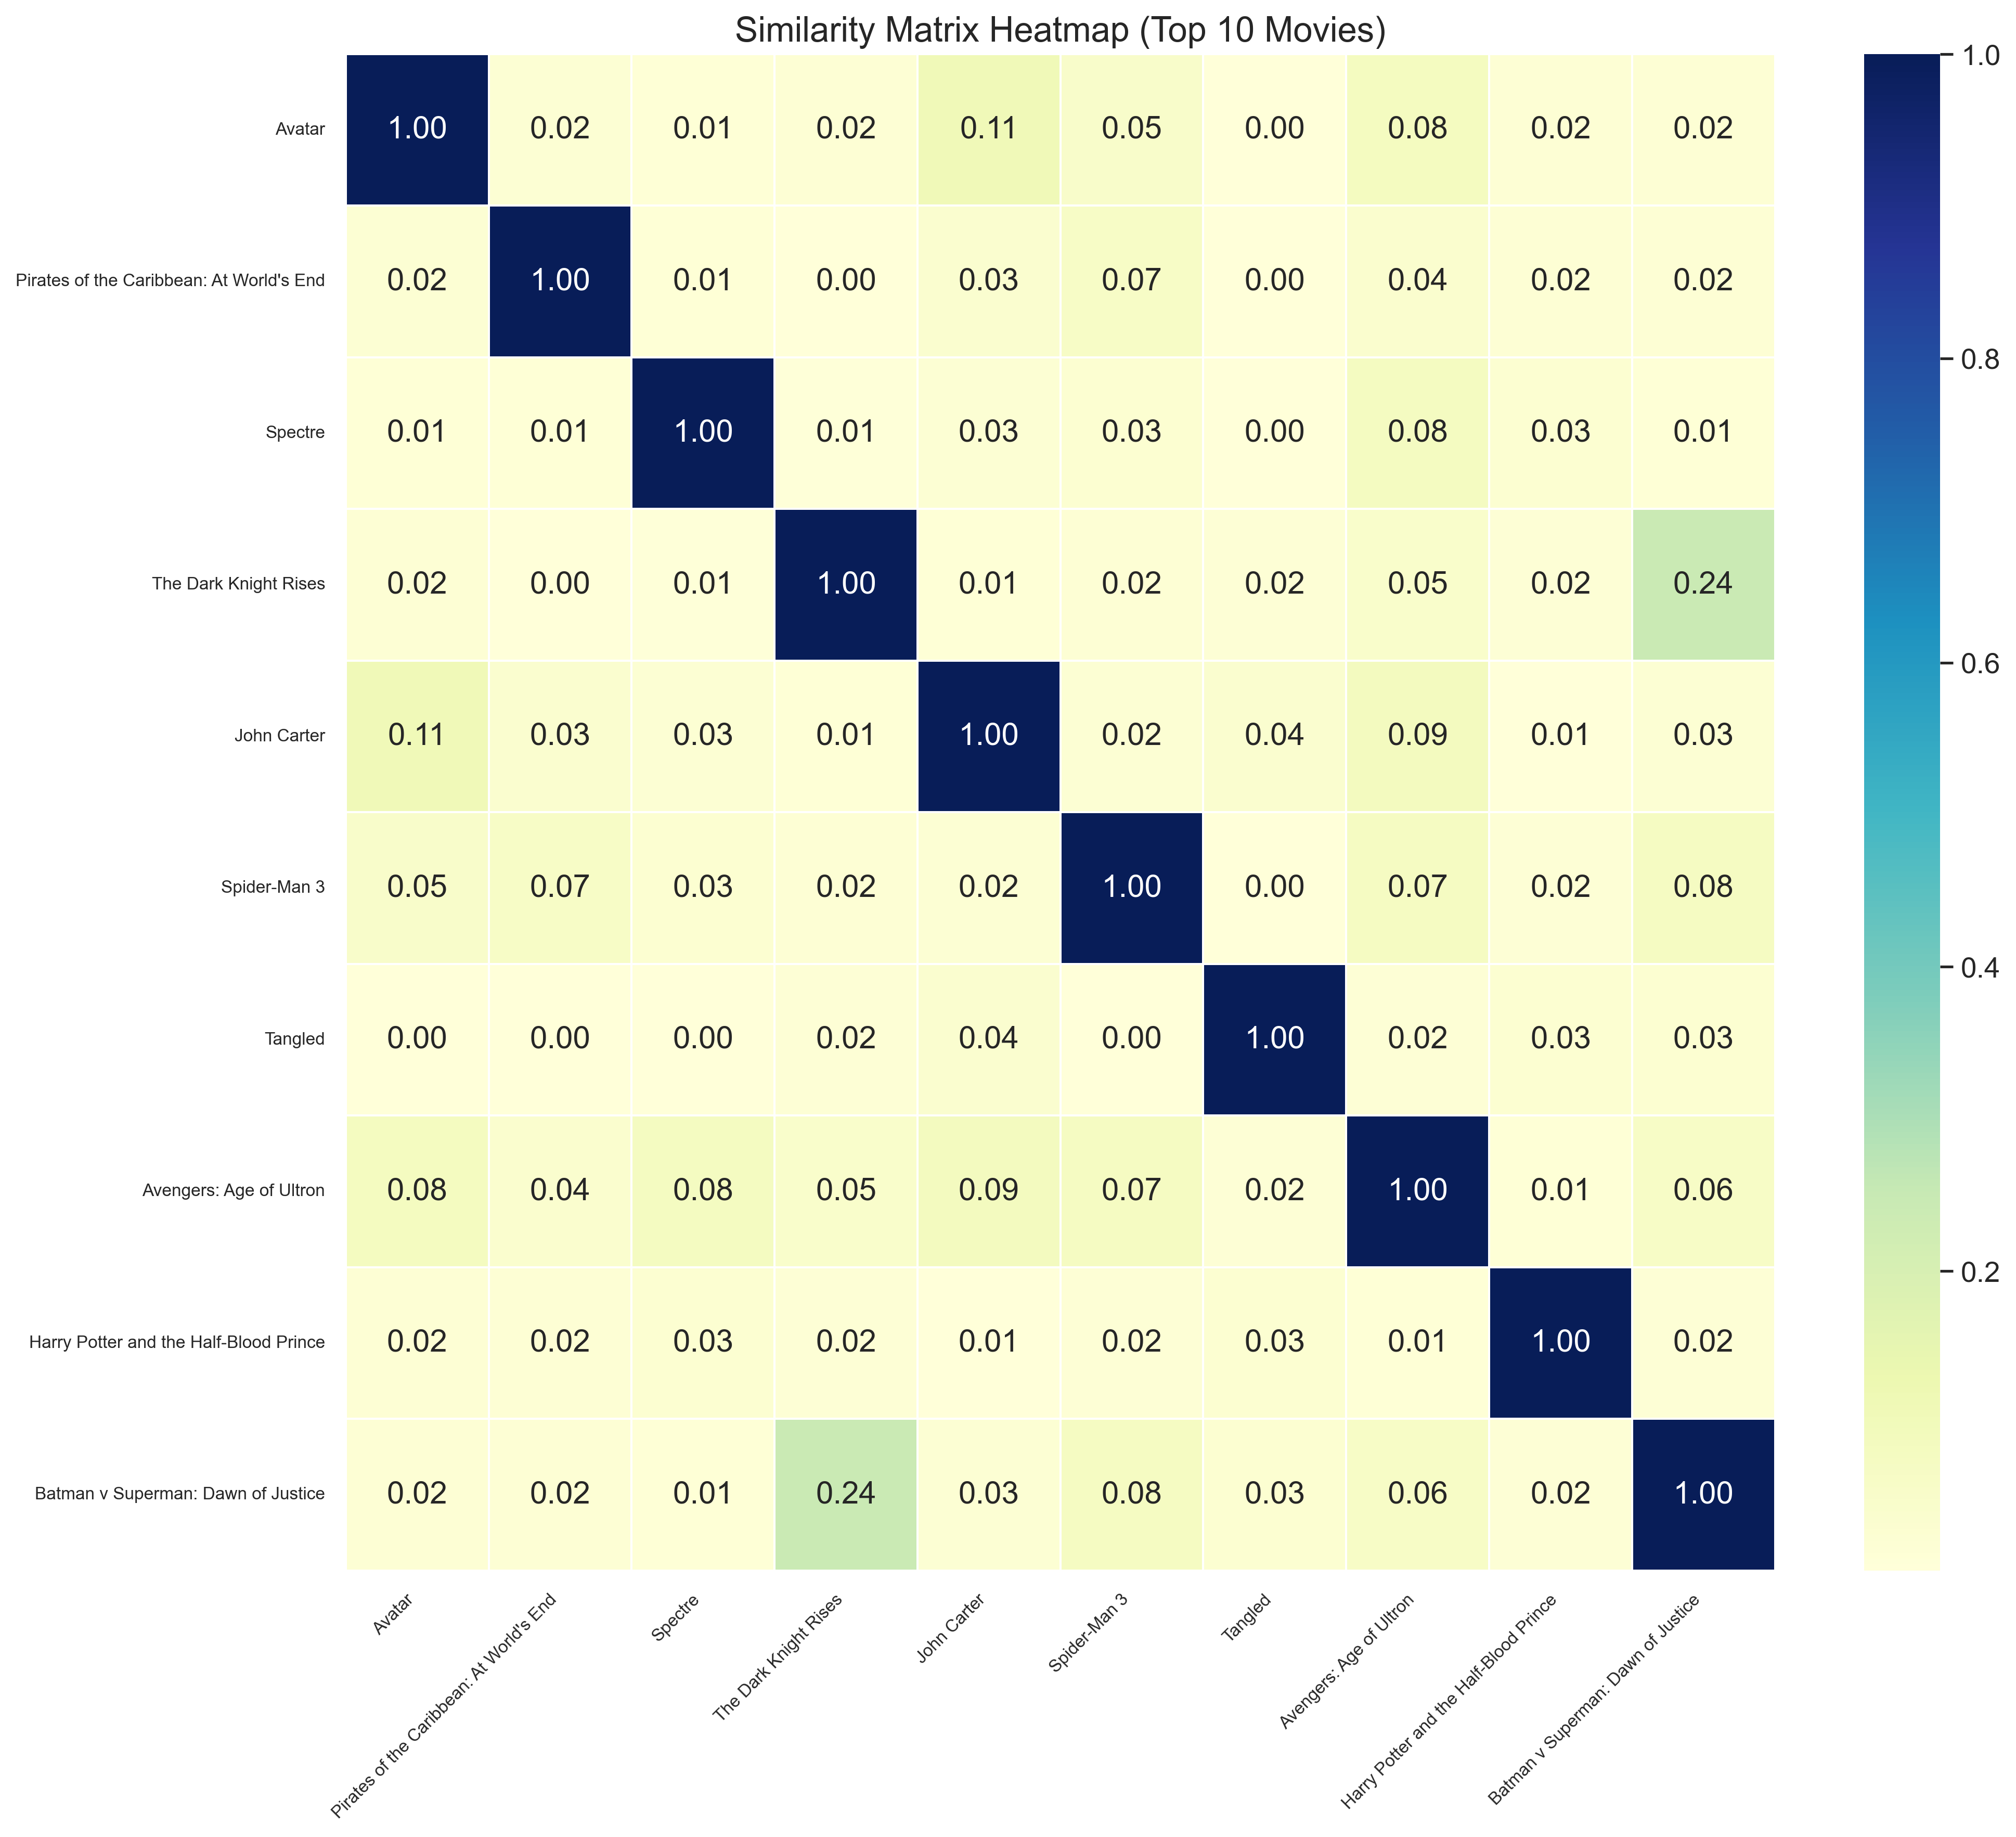
\includegraphics[width=0.9\textwidth]{static/visualizations/similarity_heatmap.png}
    \caption{Heatmap of Cosine Similarity Values Between Movies}
    \label{fig:similarity_heatmap}
\end{figure}

The heatmap reveals clusters of similar movies, with darker colors indicating higher similarity. The color scale uses the "YlGnBu" (Yellow-Green-Blue) palette, with annotation values showing the precise similarity scores. This visualization helps in understanding the underlying patterns in the recommendation system and identifying groups of movies that share similar content features.

\subsection{Recommendation Example}

Figure \ref{fig:recommendation_example} shows an example of movie recommendations generated by the system for a specific movie, along with their similarity scores.

\begin{figure}[H]
    \centering
    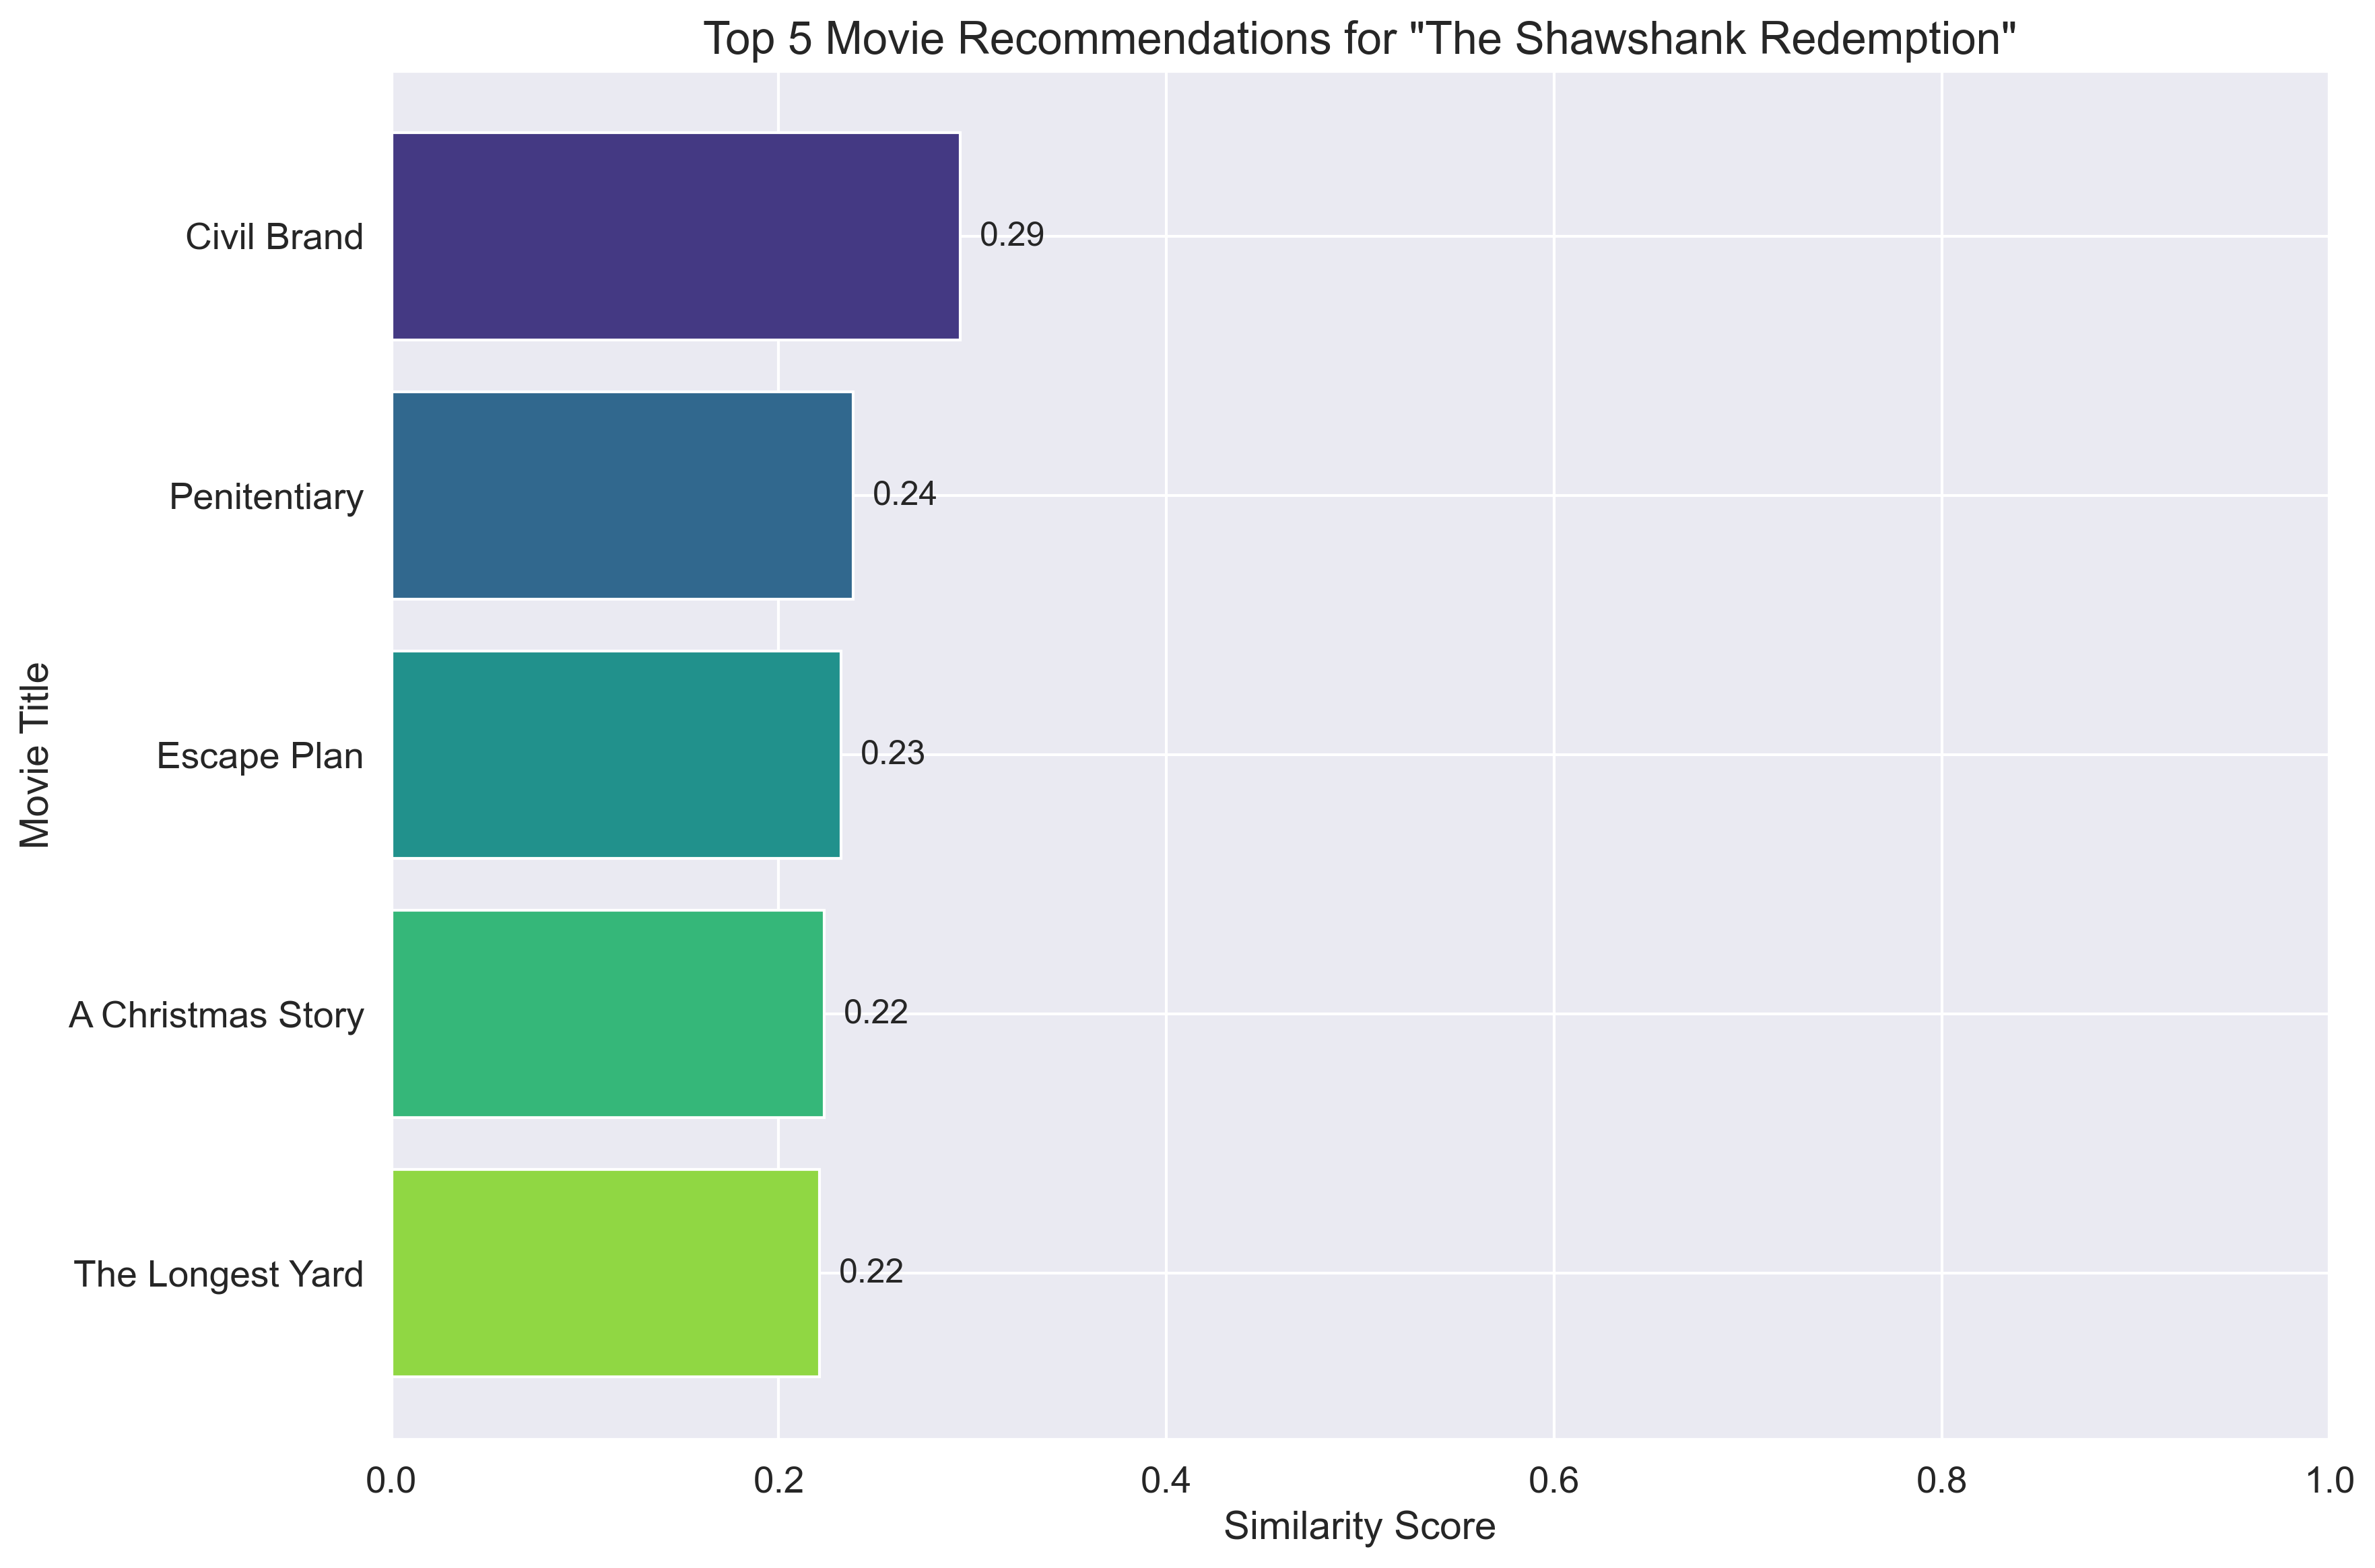
\includegraphics[width=0.9\textwidth]{static/visualizations/recommendation_example.png}
    \caption{Example of Movie Recommendations with Similarity Scores}
    \label{fig:recommendation_example}
\end{figure}

This visualization demonstrates how the system ranks similar movies based on their content features. The similarity scores provide a quantitative measure of how closely related the recommended movies are to the reference movie.

% Evaluation
\section{Evaluation}

Evaluating recommendation systems is challenging, especially for content-based systems that don't rely on user feedback. This section discusses various approaches to evaluating the movie recommendation system.

\subsection{Qualitative Evaluation}

Qualitative evaluation involves assessing the subjective quality of recommendations based on human judgment. For this system, we can evaluate recommendations by considering the following aspects:

\begin{itemize}
    \item \textbf{Relevance:} Do the recommended movies share significant content features with the reference movie?
    \item \textbf{Diversity:} Does the system recommend a diverse range of movies while maintaining relevance?
    \item \textbf{Serendipity:} Does the system recommend unexpected but interesting movies?
    \item \textbf{Explanation:} Can the system provide clear explanations for why certain movies were recommended?
\end{itemize}

Based on manual inspection of recommendation results, the system generally provides relevant recommendations that share significant content features with the reference movie. For example, when recommending movies similar to "The Dark Knight," the system suggests other superhero and action movies with similar themes and tones.

\subsection{Technical Evaluation}

From a technical perspective, the system can be evaluated based on the following criteria:

\begin{itemize}
    \item \textbf{Response Time:} The system provides recommendations within milliseconds, making it suitable for real-time applications.
    \item \textbf{Scalability:} The preprocessing approach allows the system to handle large datasets efficiently, with the similarity matrix being computed once and stored for quick lookup.
    \item \textbf{Memory Usage:} The serialized model files (movie data and similarity matrix) require reasonable storage space, making the system deployable on standard web servers.
\end{itemize}

\subsection{Limitations and Future Improvements}

The current implementation has several limitations that could be addressed in future iterations:

\begin{itemize}
    \item \textbf{Cold Start for Users:} The system doesn't account for user preferences or viewing history, making it less personalized than collaborative filtering approaches.
    \item \textbf{Limited Feature Set:} The system primarily relies on textual features and doesn't incorporate numerical features like runtime, budget, or release year.
    \item \textbf{Lack of User Feedback:} The system doesn't learn from user interactions or feedback, limiting its ability to improve over time.
\end{itemize}

Potential improvements include:

\begin{itemize}
    \item Implementing a hybrid approach that combines content-based and collaborative filtering
    \item Incorporating additional features such as movie ratings, popularity, and release date
    \item Adding user profiles to personalize recommendations based on individual preferences
    \item Implementing A/B testing to compare different recommendation algorithms
\end{itemize}

% Conclusion
\section{Conclusion}

This report has presented a comprehensive analysis of a movie recommendation system built using content-based filtering techniques, specifically TF-IDF vectorization and cosine similarity. The system successfully processes movie attributes such as genres, keywords, cast, crew, and plot descriptions to identify similarities between films and provide relevant recommendations.

The implementation includes both a backend API for generating recommendations and a frontend interface for user interaction. Visualizations of genre distribution, similarity patterns, and recommendation examples provide insights into the system's behavior and the underlying movie dataset.

While the current implementation has limitations, particularly in terms of personalization and user feedback incorporation, it demonstrates the effectiveness of content-based filtering for movie recommendations. The system provides a solid foundation that can be extended and improved in various ways to enhance recommendation quality and user experience.

In conclusion, the movie recommendation system successfully achieves its objectives of providing relevant movie suggestions based on content features, offering a responsive user interface, and implementing efficient API endpoints for data access. The visualizations and analyses presented in this report contribute to a better understanding of the system's behavior and the patterns in the movie dataset.

% References
\section{References}

\begin{enumerate}
    \item Lops, P., De Gemmis, M., \& Semeraro, G. (2011). Content-based recommender systems: State of the art and trends. In Recommender systems handbook (pp. 73-105). Springer.
    \item Ricci, F., Rokach, L., \& Shapira, B. (2011). Introduction to recommender systems handbook. In Recommender systems handbook (pp. 1-35). Springer.
    \item Scikit-learn: Machine Learning in Python, Pedregosa et al., JMLR 12, pp. 2825-2830, 2011.
    \item Flask Web Development: Developing Web Applications with Python. Miguel Grinberg. O'Reilly Media, 2018.
    \item The MovieLens Datasets: History and Context. F. Maxwell Harper and Joseph A. Konstan. ACM Transactions on Interactive Intelligent Systems, 2015.
    \item TMDB 5000 Movie Dataset. Available at: https://www.kaggle.com/datasets/tmdb/tmdb-movie-metadata
\end{enumerate}

\end{document}